\documentclass{../industrial-development}
\graphicspath{{10-quality-assurance/}}

\title{Обеспечение качества ПО}
\author{Глазовский Александр, Совин Алексей}
\date{}

\begin{document}

\begin{frame}
  \titlepage
\end{frame}



\section{Понятие качества ПО}
\begin{frame} \frametitle{Понятие качества ПО}
	\begin{block}{}
		\alert{Качество программного обеспечения} --- это совокупность характеристик ПО, относящихся к его способности удовлетворять установленные и предполагаемые потребности 
	\end{block}
\begin{itemize}
	\item Функциональность
\end{itemize}
\begin{itemize}
	\item Надежность
\end{itemize}
\begin{itemize}
	\item Удобство использования
\end{itemize}
\begin{itemize}
	\item Эффективность 
\end{itemize}
\begin{itemize}
	\item Удобство сопровождения 
\end{itemize}
\begin{itemize}
	\item Портативность  
\end{itemize}
\end{frame}

\begin{frame} \frametitle {Функциональность}
  \begin{block}{}
	\alert{Функциональность} --- способность ПО в определенных условиях решать задачи, нужные пользователям. Определяет, что именно делает ПО, какие задачи оно решает. качества 
  \end{block}
 	 \begin{itemize}
\item Функциональная пригодность --- способность решать нужный набор задач
  	\end{itemize}
   	 \begin{itemize}
  	\item Точность --- способность выдавать нужные результаты
  \end{itemize}
\begin{itemize}
	\item Способность к взаимодействию --- способность взаимодействовать с нужным набором других систем
\end{itemize}
\begin{itemize}
	\item Соответствие стандартам и правилам --- соответствие ПО имеющимся стандартам и другим регулирующим нормам
\end{itemize}
\begin{itemize}
	\item Защищенность --- способность предотвращать неавторизированный доступ к данным и программам
\end{itemize}
\end{frame}

\begin{frame} \frametitle {Надежность}
	\begin{block}{}
		\alert{Надежность} ---  способность  ПО  поддерживать  определенную  работоспособность в заданных условиях 
	\end{block}
	\begin{itemize}
		\item Зрелость, завершенность --- величина, обратная частоте отказов ПО
	\end{itemize}
	\begin{itemize}
		\item Устойчивость к отказам --- способность поддерживать заданный уровень работоспособности при отказах и нарушениях правил взаимодействия с окружением
	\end{itemize}
	\begin{itemize}
		\item Способность к восстановлению --- способность восстанавливать определенный уровень работоспособности и целостность данных после отказа
	\end{itemize}
	\begin{itemize}
		\item Соответствие стандартам надежности
	\end{itemize}
\end{frame}

\begin{frame} \frametitle {Удобство использования}
	\begin{block}{}
		\alert{Удобство использования} --- способность ПО быть удобным в обучении и использовании, а также привлекательным для пользователей 
	\end{block}
	\begin{itemize}
		\item Понятность --- показатель, обратный к усилиям, затрачиваемым пользователями на восприятие основных понятий ПО и осознание их применимости для решения своих задач
	\end{itemize}
	\begin{itemize}
		\item Удобство обучения --- показатель, обратный усилиям, затрачиваемым пользователями на обучение работе
	\end{itemize}
	\begin{itemize}
		\item Удобство работы --- показатель, обратный усилиям, предпринимаемым пользователями для решения своих задач с помощью ПО
	\end{itemize}
	\begin{itemize}
		\item Привлекательность --- способность ПО быть привлекательным для пользователей
	\end{itemize}
\end{frame}

\begin{frame} \frametitle {Эффективность}
	\begin{block}{}
		\alert{Эффективность} --- способность ПО при заданных условиях обеспечивать необходимую работоспособность по отношению к выделяемым для этого ресурсам. Можно определить ее и как отношение получаемых с помощью ПО результатов к затрачиваемым на это ресурсам всех типов 
	\end{block}
	\begin{itemize}
		\item Временная эффективность --- способность ПО выдавать ожидаемые результаты, а также обеспечивать передачу необходимого объема данных за отведенное время
	\end{itemize}
	\begin{itemize}
		\item Эффективность использования ресурсов --- способность решать нужные задачи с использованием определенных объемов ресурсов определенных видов. Имеются в виду такие ресурсы, как оперативная и долговременная память, сетевые соединения, устройства ввода и вывода и пр
	\end{itemize}
\end{frame}

\begin{frame} \frametitle {Удобство сопровождения}
	\begin{block}{}
		\alert{Удобство сопровождения} --- удобство проведения всех видов деятельности, связанных с сопровождение программ
	\end{block}
	\begin{itemize}
		\item Анализируемость --- удобство проведения анализа ошибок, дефектов и недостатков, а также удобство анализа необходимости изменений и их возможных последствий
	\end{itemize}
	\begin{itemize}
		\item Удобство внесения изменений --- показатель, обратный трудозатратам на выполнение необходимых изменений
	\end{itemize}
	\begin{itemize}
	\item Стабильность --- показатель, обратный риску возникновения неожиданных эффектов при внесении необходимых изменений
\end{itemize}
\end{frame}	

\begin{frame} \frametitle {Переносимость}
\begin{block}{}
	\alert{Переносимость} --- способность ПО сохранять работоспособность при переносе из одного окружения в другое, включая организационные, аппаратные и программные аспекты окружения	
\end{block}
	\begin{itemize}
		\item Адаптируемость --- способность ПО приспосабливаться различным окружениям без проведения для этого действий, помимо заранее предусмотренных
	\end{itemize}
	\begin{itemize}
		\item Удобство установки --- способность ПО быть установленным или развернутым в определенном окружении
	\end{itemize}
	\begin{itemize}
		\item Способность к сосуществованию --- способность ПО сосуществовать с другими программами в общем окружении, деля с ними ресурсы
	\end{itemize}
\end{frame}	

\section{Понятие управления качеством}
\begin{frame} \frametitle {Управление качеством}
\begin{block}{}
	\alert{Управление качеством} --- это совокупность мероприятий, охватывающих все технологические этапы разработки, выпуска и эксплуатации ПО, предпринимаемых на разных стадиях жизненного цикла ПО, для обеспечения требуемого уровня качества выпускаемого продукта	
\end{block}
	\begin{itemize}
	\item Верификация --- процесс оценки системы или её компонентов с целью определения удовлетворяют ли результаты текущего этапа разработки условиям, сформированным в начале этого этапа. Т.е. выполняются ли цели, сроки, задачи по разработке проекта, определенные в начале текущей фазы
\end{itemize}
	\begin{itemize}
	\item Валидация --- это определение соответствия разрабатываемого ПО ожиданиям и потребностям пользователя, требованиям к системе
\end{itemize}
\end{frame}	

\begin{frame} \frametitle{Иерархия процессов QA}
\centerline{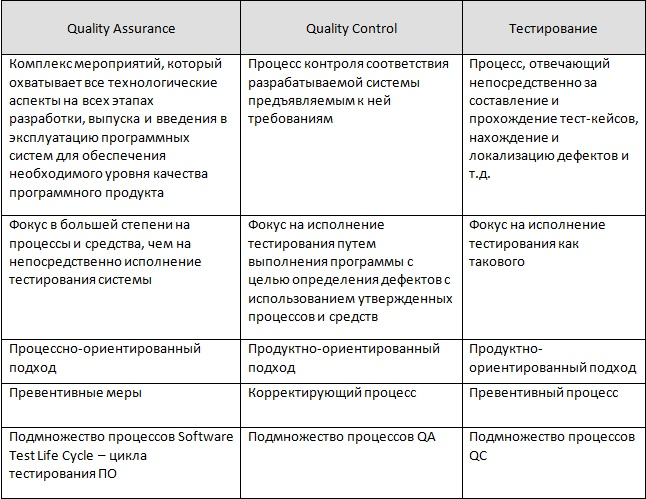
\includegraphics[height=1.0\textheight]{QA_QC.png}}
\end{frame}

\begin{frame} \frametitle{Иерархия процессов QA}
\begin{flushleft}
Quality Assurance обеспечивает правильность и предсказуемость процесса, в то время как Quality Control предполагает контроль соблюдения требований. Тестирование же, в свою очередь, обеспечивает сбор статистических данных и внесение их в документы, созданные в рамках QC-процесса
\end{flushleft}
\centerline{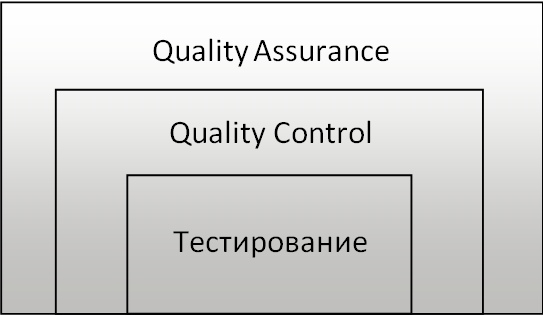
\includegraphics[height=0.7\textheight]{QA_QC2.png}}
\end{frame}

\begin{frame} \frametitle{Пример на велосипеде}
\begin{itemize}
\item с помощью тестирования мы можем определить, работают ли все детали и сам велосипед в целом так, как мы ожидаем. Из правильных ли материалов он сделан, с применением нужных методик и инструментов или нет. То есть, подразумевается, что тестируемый объект уже существует.
\item задачей же QA является обеспечение соответствия всех этапов конструирования нашего велосипеда определенным стандартам качества, начиная с планирования и создания чертежей и заканчивая сборкой уже готового велосипеда. То есть, качеству объекта внимание уделяется еще до создания самого объекта.
\end{itemize}
\end{frame}

\section{Модели QA}
\begin{frame} \frametitle{Каскадная модель}
\begin{flushleft}
	Самой старой и известной моделью построения многоуровневого процесса разработки является каскадная (или попросту водопадная) модель: в ней каждый этап разработки, соответствующий стадии жизненного цикла ПО, продолжает предыдущий. То есть, для того, чтобы перейти на новый этап, мы полностью должны завершить текущий.
	
	Каскадная модель проста и понятна, но не так практична как раньше. В условиях динамично изменяющихся требований, строго структурированный процесс может из преимущества превратиться в помеху на пути успешного завершения разработки системы. Поэтому сегодня водопадная модель применяется преимущественно крупными компаниями для больших и сложных проектов, которые предполагают всеобъемлющий контроль рисков
\end{flushleft}
\end{frame}

\begin{frame} \frametitle{Плюсы каскадной модели}
\begin{itemize}
\item Полное документирование каждого этапа
\item Четкое планирование сроков и затрат
\item Прозрачность процессов для заказчика
\end{itemize}
\end{frame}

\begin{frame} \frametitle{Минусы каскадной модели}
\begin{itemize}
	\item Необходимость утверждения полного объема требований к системе еще на первом этапе
	\item В случае необходимости внесения изменений требований позднее – возврат к первой стадии и переделка заново всей проделанной работы
	\item Увеличение затрат средств и времени в случае необходимости изменения требований
\end{itemize}
\end{frame}

\begin{frame} \frametitle{Использование каскадной модели}
\begin{itemize}
	\item В проектах с четко определенными требованиями, для которых не предусматривается их изменений в процессе разработки
	\item Для проектов, которые мигрируют с одной платформы на другую. То есть, требования остаются те же, меняется только системное окружение и/или язык программирования
	\item Когда от компании-разработчика не требуется проводить тестирования – к примеру, его обеспечением займется сам заказчик или сторонняя фирма
\end{itemize}
\end{frame}

\begin{frame} \frametitle{V-модель}
\begin{flushleft}
V-модель – это улучшенная версия классической каскадной модели. Здесь на каждом этапе происходит контроль текущего процесса. В этой модели тестирование начинается еще со стадии написания требований, причем для каждого последующего этапа предусмотрен свой уровень тестового покрытия. Для каждого уровня тестирования разрабатывается отдельный тест-план.

В V-модели каждому этапу проектирования и разработки системы соответствует отдельный уровень тестирования. Здесь процесс разработки представлен нисходящей последовательностью в левой части условной буквы V, а стадии тестирования – на ее правом ребре.
\end{flushleft}
\end{frame}

\begin{frame} \frametitle{Плюсы V-модели}
\begin{itemize}
	\item Строгая этапизация
	\item Планирование тестирования и верификация системы производятся на ранних этапах
	\item Улучшенный, по сравнению с каскадной моделью, тайм-менеджмент
	\item Промежуточное тестирование
\end{itemize}
\end{frame}

\begin{frame} \frametitle{Минусы V-модели}
\begin{itemize}
	\item Недостаточная гибкость модели
	\item Собственно создание программы происходит на этапе написания кода, то есть уже в середине процесса разработки
	\item Недостаточный анализ рисков
	\item Нет работы с параллельными событиями и возможности динамического внесения изменений
\end{itemize}
\end{frame}

\begin{frame} \frametitle{Использование V-модели}
\begin{itemize}
	\item В проектах, в которых существуют временные и финансовые ограничения
	\item Для задач, которые предполагают более широкое, по сравнению с каскадной моделью, тестовое покрытие
\end{itemize}
\end{frame}

\begin{frame} \frametitle{Спиральная модель}
\begin{flushleft}
	Спиральная модель представляет шаблон процесса разработки ПО, который сочетает идеи итеративной и каскадной моделей. Суть ее в том, что весь процесс создания конечного продукта представлен в виде условной плоскости, разбитой на 4 сектора, каждый из которых представляет отдельные этапы его разработки: определение целей, оценка рисков, разработка и тестирование, планирование новой итерации.
	
	В спиральной модели жизненный путь разрабатываемого продукта изображается в виде спирали, которая, начавшись на этапе планирования, раскручивается с прохождением каждого следующего шага. Таким образом, на выходе из очередного витка мы должны получить готовый протестированный прототип, который дополняет существующий билд. Прототип, удовлетворяющий всем требованиям – готов к релизу.
\end{flushleft}
\end{frame}

\begin{frame} \frametitle{Оценка рисков в спиральной модели}
\begin{flushleft}
	Главная особенность спиральной модели – концентрация на возможных рисках. Для их оценки даже выделена соответствующая стадия. Основные типы рисков, которые могут возникнуть в процессе разработки ПО
\end{flushleft}
\begin{itemize}
\item Нереалистичный бюджет и сроки
\item Дефицит специалистов
\item Частые изменения требований
\item Чрезмерная оптимизация
\item Низкая производительность системы
\item Несоответствие уровня квалификации специалистов разных отделов
\end{itemize}
\end{frame}

\begin{frame} \frametitle{Плюсы спиральной модели}
\begin{itemize}
	\item Улучшенный анализ рисков
	\item Хорошая документация процесса разработки
	\item Гибкость – возможность внесения изменений и добавления новой функциональности даже на относительно поздних этапах
	\item Раннее создание рабочих прототипов
\end{itemize}
\end{frame}

\begin{frame} \frametitle{Минусы спиральной модели}
\begin{itemize}
\item Может быть достаточно дорогой в использовании
\item Управление рисками требует привлечения высококлассных специалистов
\item Успех процесса в большой степени зависит от стадии анализа рисков
\item Не подходит для небольших проектов
\end{itemize}
\end{frame}

\begin{frame} \frametitle{Использование спиральной модели}
\begin{itemize}
\item В проектах, в которых важен анализ рисков и затрат
\item Крупные долгосрочные проекты с отсутствием четких требований или вероятностью их динамического изменения
\item При разработке новой линейки продуктов
\end{itemize}
\end{frame}

\begin{frame} \frametitle{Итеративная модель}
\begin{flushleft}
	Не все модели жизненного цикла последовательны. Существуют также итеративные модели, в которых используется другой подход. Вместо одной продолжительной последовательности действий здесь весь жизненный цикл продукта разбит на ряд отдельных мини-циклов. Причем каждый из них состоит из все тех же базовых стадий модели жизненного цикла. Эти мини-циклы называются итерациями. В каждой из итераций происходит разработка отдельного компонента системы, после чего этот компонент добавляется к уже ранее разработанному функционалу.
	
	Итеративная модель не предполагает полного объема требований для начала работ над продуктом. Разработка программы может начинаться с требований к части функционала, которые могут впоследствии дополняться и изменяться.  Процесс повторяется, обеспечивая создание новой версии продукта для каждого цикла.
\end{flushleft}
\end{frame}

\begin{frame} \frametitle{Цикл PDCA}
\begin{flushleft}
В несколько упрощенном виде, итеративная модель состоит из четырех основных стадий, которые повторяются в каждой из итераций (plan-do-check-act):
\end{flushleft}
\begin{itemize}
\item Определение и анализ требований
\item Дизайн и проектирование – согласно требованиями. Причем дизайн может как разрабатываться отдельно для данной функциональности, так и дополнять уже существующий
\item Разработка и тестирование – кодирование, интеграция и тестирование нового компонента
\item Фаза ревью – оценка, пересмотр текущих требований и предложения дополнений к ним
\end{itemize}
\end{frame}

\begin{frame} \frametitle{Плюсы итеративной модели}
\begin{itemize}
\item Раннее создание работающего ПО
\item Гибкость – готовность к изменению требований на любом этапе разработки
\item Каждая итерация – маленький этап, для которого тестирование и анализ рисков обеспечить проще, чем для всего жизненного цикла продукта
\end{itemize}
\end{frame}

\begin{frame} \frametitle{Минусы итеративной модели}
\begin{itemize}
\item Каждая фаза – самостоятельна, отдельные итерации не накладываются
\item Могут возникнуть проблемы с реализацией общей архитектуры системы, поскольку не все требования известны к началу проектирования
\end{itemize}
\end{frame}

\begin{frame} \frametitle{Использование итеративной модели}
\begin{itemize}
\item Для крупных проектов
\item Когда известны, по крайней мере, ключевые требования
\item Когда требования к проекту могут меняться в процессе разработки
\end{itemize}
\end{frame}

\begin{thebibliography}{99}
\bibitem{SQA-Galin} Galin, Daniel, Software quality assurance: from theory to implementation / Daniel Galin, 2004."--- 590с.: ил.
\end{thebibliography}

\end{document}